\documentclass[12pt,a4paper]{article}
 \usepackage[italian]{babel}
 \usepackage[latin1]{inputenc}
 \usepackage{verbatim}
 \usepackage{amsmath}
 \usepackage{graphicx}
 \usepackage{url}
 \usepackage{geometry}
 \usepackage{color}
 \usepackage{subfigure}
 \usepackage{multirow}
 \newenvironment{sistema}%
  {\left\lbrace\begin{array}{@{}l@{}}}%
  {\end{array}\right.}
 
 \geometry{a4paper,top=3cm,bottom=3cm,left=1.5cm,right=1.5cm,heightrounded,bindingoffset=1cm}
 
 \begin{document}
 	\title{Modello matematico con tre masse e tre molle smorzate} \author{Matteo Bolognese}
 	\date{23/11/2019}
 	\maketitle
 	
 \section{Introduzione}
	La misura sperimentale della costante elastica dinamica di un materiale $K(\omega)$ per mezzo di un martello strumentato \'e stata effettuata con diverse configurazioni di misura. Una delle pi\'u semplici, rappresentata in \figurename~\ref{fig:Phisical-system}, prevede il posizionamento di una piastra di carico sul campione a sua volta poggiato al suolo. La piastra di carico viene colpita con il martello strumentato e uno o pi\'u accelerometri misurano l'accelerazione della piastra e/o del suolo a seconda degli intenti della misura.
	
	
	\begin{figure}
		\centering	
		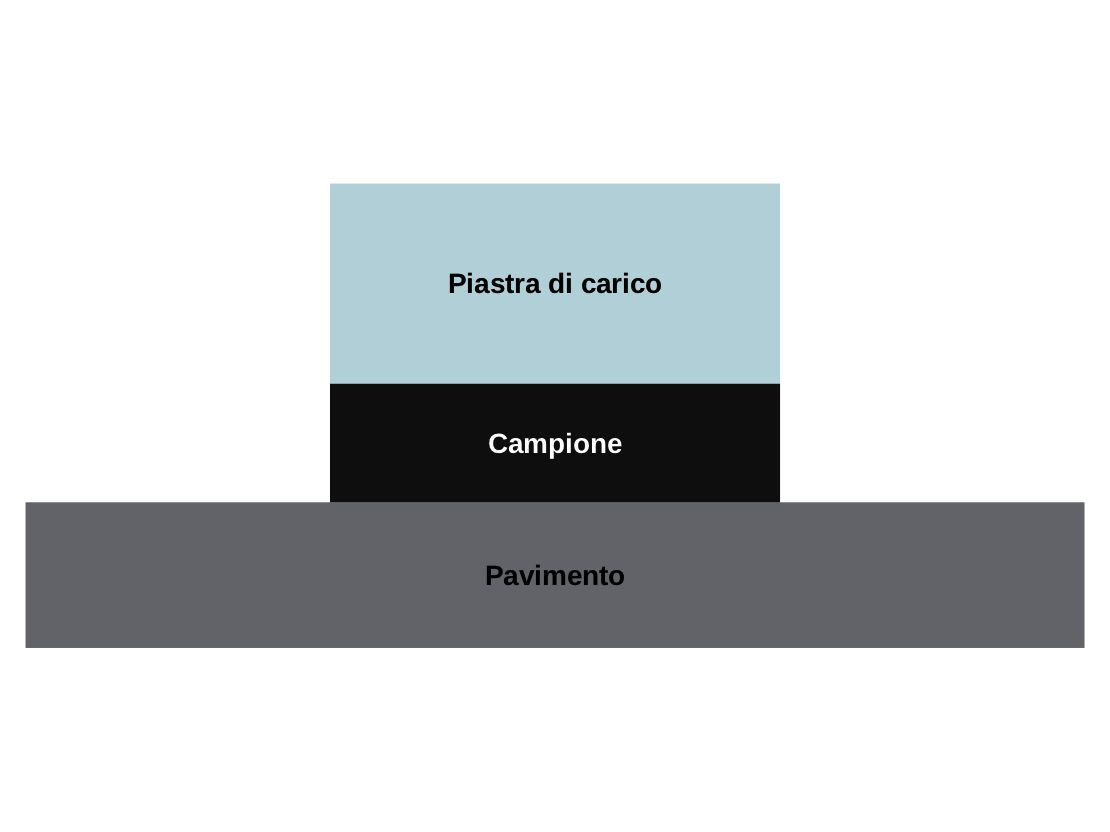
\includegraphics[width=13cm]{Phisical-system.jpg}
		\caption{Configurazione sperimentale.}
		\label{fig:Phisical-system}
	\end{figure}
 	
 \section{Misure in laboratorio}
 Anche al fine di calibrare la catena strumentale messa a punto finora, presso l’Università di Reggio Calabria il Prof. Praticò curerà la realizzazione di campioni di conglomerato bituminoso variando i seguenti parametri:
    • quantitativo di polverino di gomma impiegato;
    • la tipologia di lavorazione (Wet o Dry);
    • la curva granulometrica;
    • frazione dei vuoti;
in modo tale da coprire il più possibile il range di variabilità.
I campioni realizzati verranno quindi inviati a Pisa presso iPool s.r.l. e analizzati tramite l’apparato sperimentale in fase di sviluppo. Le prove avranno la duplice valenza di calibrazione tramite confronto con metodi di misura tradizionali (ad esempio la prova triassiale) e di riferimento per valutare eventuali discordanze tra misure in laboratorio e misure in sito. Terminate le prove presso iPool s.r.l i campioni potranno essere inviati all’Università  di Reggio Calabria per essere sottoposti a ulteriori prove di laboratorio anche di carattere distruttivo.

 \end{document}